\section{LuRaCs-Xe}
\begin{center}
    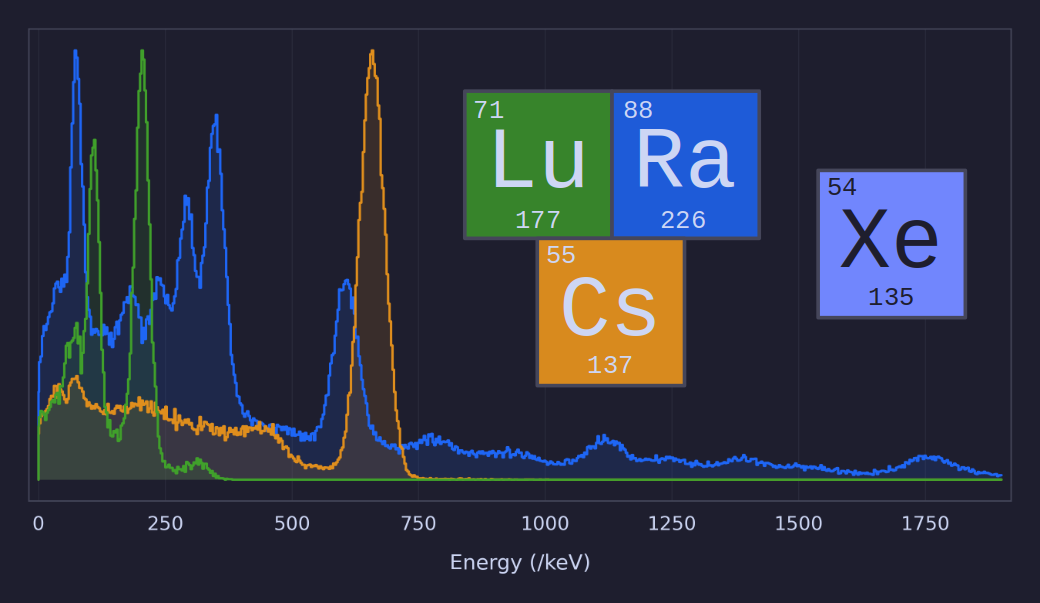
\includegraphics[width=.6\linewidth]{images/appendix/LuRaCs-Xe.png}
\end{center}
LuRaCs-Xe is a supplementary resource repository developed to accompany the main LuRaCs application. It provides a collection of example datasets, reference materials, and other resources intended to support the use, testing, and further development of LuRaCs. This resource is continually updated independently of the main application. Each component contains a README-file that provides information about the specific resource.

By bringing these resources together in a common repository, LuRaCs-Xe aims to facilitate reproducible analysis, provide practical examples for new users, and support the development and evaluation of analytical methods.

It currently contains the following sections:
\begin{itemize}
    \item \texttt{example\_spectra}: Spectrum files from measurements we have conducted with a verity of sources and detectors.
    \item \texttt{roi\_references}: Predefined ROIs for common nuclides for use with LuRaCs. Especially useful when using spectrogram ROIs as the bounds have been determined from peaks with good statistics.
    \item \texttt{response\_matrices}: Simulated detector response matrices for use in the spectrum deconvolution tool in LuRaCs.
\end{itemize}